%%% kswrapfig 사용설명서와 예제

\documentclass[a4paper,nanum]{oblivoir}

\usepackage{tabu}
\usepackage{xcolor}
\usepackage{tikz}
\usepackage[framemethod=tikz]{mdframed}

%\ifxetex
%\defaultfontfeatures{Mapping=tex-text}
%\setkormainfont{맑은 고딕}\hangulmarks
%\fi

\usepackage[dbl4x6]{fapapersize}

\usepackage[insbox]{kswrapfig}

%%% 테스트용 텍스트
\newcommand\LongText{%
TeX(텍)은 탁월한 조판 프로그래밍 언어입니다. 한글 텍 사용자 그룹은 텍과 그 파생 매크로 집합인 LaTeX, ConTeXt, AMSLaTeX 등을 사용하여 논문을 작성하거나 프로그래밍하거나 책을 만들거나 하는 일을 하는 사용자들의 모임입니다.	 텍에 대하여 궁금하시면 TeX 페이지를, LaTeX에 대해서는 LaTeX 페이지를 참조하십시오. 텍을 처음 사용하신다면 처음 시작하기를 읽어보시기 바랍니다. 이곳에서는 질답 게시판을 통하여 의견을 나눌 수 있고 위키나 기고 게시판을 통하여 유용한 지식을 다른 사람과 공유할 수 있습니다. Happy TeX'ing.
}

\newcommand\ShortText{%
TeX(텍)은 탁월한 조판 프로그래밍 언어입니다.
한글 텍 사용자 그룹은 텍과 그 파생 매크로 집합인
}

\newcommand\LongListText{%
\item TeX(텍)은 탁월한 조판 프로그래밍 언어입니다. 
\item 텍을 처음 사용하신다면 처음 시작하기를 읽어보시기 바랍니다. 이곳에서는 질답 게시판을 통하여 의견을 나눌 수 있고 위키나 기고 게시판을 통하여 유용한 지식을 다른 사람과 공유할 수 있습니다.
\item 한글 텍 사용자 그룹은 텍과 그 파생 매크로 집합인 LaTeX, ConTeXt, AMSLaTeX 등을 사용하여 논문을 작성하거나 프로그래밍하거나 책을 만들거나 하는 일을 하는 사용자들의 모임입니다.
}

\newcommand\ShortListText{%
\item TeX(텍)은 탁월한 조판 프로그래밍 언어입니다. 
\item Happy TeX'ing.
}

\begin{document}

\title{kswrapfig.sty}
\author{Karnes}
\date{{\small version 0.004}\\ \today}

\maketitle

\begin{abstract}
kswrapfig 패키지는 원래 kstextflow라는 이름이었다. 이름을 바꾸고 기능을 추가한 후 2012년
한국텍학회 학술대회\footnote{\url{http://conf.ktug.or.kr/2012/}}에서 발표하였다.
이 패키지는 picins\footnote{picins는 \TeX\,Live에 포함되지 않으며 이 패키지와 함께 동작하게 하기 
위해서 원본 picins에 약간의 수정을 가해야 했다. 그런 까닭에 이 패키지 안에 picins 전체를 포함한다. 다만 picins가 라이선스에 대해서 아무런 정보를 제공하지 않는 모호함이 있다. kswrapfig은 단순히 \emph{free}이다.}, picinpar 패키지를 이용하여 문단 가운데 그림을 두고 그 주위로 텍스트가 흐르게 한다.
그림과 텍스트 사이의 간격과 위치를 조절하는 옵션을 제공하는 것이 이 패키지의 목적이다.
\verb|\kswrapfig| 명령과 \verb|\kswrapfigline| 두 개의 명령을 사용할 수 있다.

이전 버전에서 이 패키지는 memoir/oblivoir에서만 동작하였으나 0.002.3버전부터 일반 클래스에서도
동작하도록 수정하였다. 따라서 article 등의 클래스에서도 쓸 수 있다.
%\footnote{%
%	이 패키지는 memoir 또는 oblivoir에서만 함께 쓰일 수 있다.}
\end{abstract}

\renewcommand*\contentsname{}
\maxtocdepth{paragraph}
\begin{mdframed}[skipabove=\onelineskip,frametitle=\textcolor{gray!90}{차\ \ \ \ 례},%
	frametitlealignment=\centering,
	frametitlebackgroundcolor=blue!15,
	frametitlebelowskip=5pt,
	frametitlerulecolor=gray,
	frametitlerulewidth=.4pt,
	frametitlerule=true,
	innertopmargin=-1.2\onelineskip,
	backgroundcolor=red!10,
	splittopskip=12pt,
	splitbottomskip=10pt,
	needspace=\onelineskip,
	outerlinewidth=1pt,
	outerlinecolor=gray!60,
	middlelinecolor=gray!60,
	innerlinecolor=gray!60,
]
\small
\tableofcontents*
\end{mdframed}

\clearpage

\section{초 간단명료 설명}

\paragraph{\texttt{\textbackslash}kswrapfig 명령}

\begin{boxedverbatim}
\kswrapfig[Options=keyval]{Figure}{TEXT}
\end{boxedverbatim}

옵션에 올 수 있는 \textit{keyval}은 다음과 같다.
\begin{enumerate}\tightlist
\item \verb|Pos= |, r 또는 l.
\item \verb|Width= |, 길이. 5cm, 4cm, etc. 그림의 가로폭이다. 이 패키지는 오직 그림의 width만으로 조판한다. scale 등은 쓰지 않으므로 주의할 것. 기본값은 무조건 5cm임.
\item \verb|InPos= |, r, c 또는 l. 그림 자체의 내부 정렬 방식을 가리키는데, 실제로 그림 위치를 지정하는 다른 옵션이 많으므로 웬만하면 무시하는 것이 좋다.
\item \verb|Sep= |, 그림과 텍스트 사이의 간격. 길이 단위로 준다. 예를 들면 10pt, 20pt 등등.
\item \verb|Indent= |, 그림의 가로 위치(horizontal position)를 잡기 위한 들여쓰기 값. 
\item \verb|Lower= |, 그림의 세로 위치(vertical position)를 잡기 위한 내려찍기 값.
\item \verb|Caption={caption text}|, 그림에 캡션을 붙여야 할 때 쓴다.
\item \verb|LastLineSkip= |, 문단과 그림이 식자된 후 마지막 줄과 다음 문단 사이의 거리를 임의로 조절할 수 있다. 길이값을 준다.
\item \verb|FirstLineSkip= |, 길이. 문단이 시작하는 위치의 수직 길이를 튜닝하게 해준다.
\item \verb|List= |, 텍스트 부분이 평문단이 아니라 리스트 환경일 때. List=enumerate 과 같은 방식으로 지정한다.
\item \verb|VAdjust= |, 길이. 행간의 변화 등으로 원치않는 행수만큼 텍스트가 흐를 때 이를 조정하기 위한 값을 지정한다.
\item \verb|UseBox = |, true or false. 이 값이 true가 되면 첫번째 인자에 그림 이름이 오는 것이 아니라 \dotemph{임의의 텍스트}가 온다. 예를 들어 tabular 등이 올 수 있게 된다. false로서 그림 파일 이름을 적는 것이 디폴트.
\end{enumerate}

문단이 리스트 환경일 경우에도 쓸 수 있으며 리스트 환경으로 제공되는 텍스트의 분량에 따라 적절한 배열을 해준다.
단, 리스트 환경은 무조건 compact list로 조판된다.

\paragraph{\texttt{\textbackslash}kswrapfigline 명령}

\begin{boxedverbatim}
\kswrapfigline[Line=n,<Other keyval Options>]{Figure}{TEXT}
\end{boxedverbatim}

이 명령은 문단의 $n$라인이 지난 후에 그림이 찍히도록 한다. \verb|\kswrapfig|의 명령과 같은 옵션을 가지지만
다음 옵션은 사용되지 않는다.
\begin{enumerate}\tightlist
\item \verb|List= |. list 환경과는 함께 쓰지 않는다.\footnote{list 환경의 $n$라인을 먼저 찍는다는 것은 불필요해보인다.}
따라서 \verb|List= | 옵션은 무의미하다. 이 명령에서는 \verb|InPos| 옵션이 동작하지 않는다.
\item \verb|InPos= |. 내부 박스는 언제나 가운데 정렬로 식자하므로 이 옵션은 disable.
%\item \verb|VAdjust= |. \verb|\kswrapfig|과 박스를 두는 방식이 다르기 때문에 이 옵션이 필요한 상황이 거의 발생하지 않는다.
\end{enumerate}
다음 옵션이 추가적으로 동작한다.
\begin{enumerate}\tightlist
\item \verb|Pos= |, \verb|\kswrapfig|의 l, r 외에 c 옵션을 하나 더 이용할 수 있다. 이것은 문단 한가운데 그림 박스를 만들고 그 주위로 텍스트를 플로우시킨다.
\item \verb|Line= |, 숫자. 문단의 상단에 보낼 행수를 적는다.
\item \verb|CaptionName= |, figure or table. \verb|Caption|이 주어지고 \verb|UseBox=true|일 경우에 이 값을 table로 하면 캡션 이름이 `그림 1: '이 아니라 `표 1: '로 찍힌다.\footnote{캡션 이름을 바꾸는 것은 \texttt{\textbackslash kswrapfig}에서는 되지 않으며 \texttt{\textbackslash kswrapfigline}에서만 동작한다.}
\end{enumerate}

\paragraph{\texttt{\textbackslash ksinsbox} 명령}

\verb|\usepackage[insbox]{kswrapfig}| \\
또는 \verb|\usepackage[insboxonly]{kswrapfig}|

\begin{boxedverbatim}
\ksinsbox[<l,r,c>][<num>]{box_codes}
\end{boxedverbatim}
\begin{enumerate}
\item 그림의 위치.
\item 그림 이전에 식자할 문단의 행 수. 단, 그림 위치가 \verb|c|일 때는 이 옵션이 의미가 없다.
\item \verb|box_codes|에는 무엇이든 올 수 있다. \verb|\parbox|, \verb|tabular|, \verb|\includegraphics| 등. 그러므로 그림을 넣을 것이라면 \verb|\includegraphics|를 써서 지정한다.
\end{enumerate}


\clearpage
\section{그림과 문단을 배치하기}

\paragraph{심플하게}
\begin{boxedverbatim}
\kswrapfig{fig1}{\LongText}
\end{boxedverbatim}

\kswrapfig{fig1}{\LongText}

\paragraph{그림을 문단의 오른쪽으로}
\begin{boxedverbatim}
\kswrapfig[Pos=r]{fig1}{\LongText}
\end{boxedverbatim}

\kswrapfig[Pos=r]{fig1}{\LongText}

\paragraph{두 문단 이상일 때 문제없음}
\begin{boxedverbatim}
\kswrapfig{fig1}{\ShortText\par\LongText}
\end{boxedverbatim}

\kswrapfig{fig1}{\ShortText\par\LongText}

\paragraph{그림 크기를 조절 Width}
\begin{boxedverbatim}
\kswrapfig[Pos=r,Width=1cm]{fig1}{\LongText}
\end{boxedverbatim}

\kswrapfig[Pos=r,Width=1cm]{fig1}{\LongText}

\paragraph{그림과 텍스트 사이의 간격을 조절 Sep}

\begin{boxedverbatim}
\kswrapfig[Width=5cm,Sep=2em]{fig1}{\LongText}
\end{boxedverbatim}

\kswrapfig[Width=5cm,Sep=2em]{fig1}{\LongText}

\paragraph{그림 수평 위치를 조절 Indent}
마이너스 인덴트를 주는 경우 현재 판면의 범위를 벗어나서 놓이지 않는다. 즉 여백 영역 안에서만 Indent가
작용한다. 만약 판면 영역 바깥까지 그림을 끌어내어야 할 필요가 있다면 \pageref{sec:other} 페이지의 \titleref{sec:other} 항목을 보라.

\begin{boxedverbatim}
\kswrapfig[Width=5cm,Indent=-2em]{fig1}{\LongText}
\end{boxedverbatim}

\kswrapfig[Width=5cm,Indent=-2em]{fig1}{\LongText}

\paragraph{그림 수직 위치를 조절 Lower}
\begin{boxedverbatim}
\kswrapfig[Width=5cm,Lower=2em]{fig1}{\LongText}
\end{boxedverbatim}

\kswrapfig[Width=5cm,Lower=2em]{fig1}{\LongText}

\paragraph{Indent, Sep, Lower로 수평 간격, 수직 간격을 모두 적용}

\begin{boxedverbatim}
\kswrapfig[Width=5cm,Indent=-2em, Lower=-2em, Sep=2em]
{fig1}{\LongText}
\end{boxedverbatim}

\kswrapfig[Width=5cm,Indent=-2em, Lower=-2em, Sep=2em]{fig1}{\LongText}


\paragraph{문단 전후의 행간격을 늘리거나 줄이는 트릭 FirstLineSkip, LastLineSkip}
kswrapfig으로 조판을 하다보면 경우에 따라 의도하지 않은 문단 사이의 간격이
생겨날 수 있다. 이것을 미세조절하는 데 다음과 같은 트릭을 쓴다.

\begin{boxedverbatim}
\kswrapfig[Width=5cm,LastLineSkip=\onelineskip]{fig1}{\LongText}
\end{boxedverbatim}

\kswrapfig[Width=5cm,LastLineSkip=\onelineskip]{fig1}{\LongText}

\kswrapfig[Pos=r]{fig1}{%
 \LongText
}

\vskip4\onelineskip

\begin{boxedverbatim}
\kswrapfig[Width=5cm,FirstLineSkip=\onelineskip]{fig1}{\LongText}
\end{boxedverbatim}

\kswrapfig[Width=5cm]{fig1}{\LongText}
\kswrapfig[Width=5cm,FirstLineSkip=\onelineskip]{fig1}{\LongText}

\paragraph{VAdjust를 통한 긴 텍스트 흐름의 조절}
행간(baselinestretch)이 달라지면 때때로 텍스트의 흐름이 부자연스러워지는 경우가 있다.
이를 위하여 그림 박스의 세로 길이를 조절할 수 있게 하였다. 아래 첫번째 샘플은 기본 옵션으로 한 것인데
텍스트가 긴 줄로 바뀌는 부분을 한 줄 뒤로 한 것이 그 다음 샘플이다.\footnote{VAdjust는 Long Text에서만
효과가 있다.}

\begin{boxedverbatim}
\kswrapfig[Width=4cm]{fig1}{\LongText}
\end{boxedverbatim}

\begin{Spacing}{1.0}
\kswrapfig[Width=4cm]{fig1}{\LongText}
\end{Spacing}

\begin{boxedverbatim}
\kswrapfig[Width=4cm,VAdjust=\onelineskip]{fig1}{\LongText}
\end{boxedverbatim}

\begin{Spacing}{1.0}
\kswrapfig[Width=4cm,VAdjust=\onelineskip]{fig1}{\LongText}
\end{Spacing}

\paragraph{짧은 문단}
\begin{boxedverbatim}
\kswrapfig[Pos=l,Width=5cm,LastLineSkip=10pt]{fig1}{\ShortText}

\kswrapfig[Pos=r,Width=5cm,Sep=1em]{fig1}{\ShortText}
\end{boxedverbatim}


\kswrapfig[Pos=l,Width=4cm,LastLineSkip=10pt]{fig1}{%
 \ShortText
}

\kswrapfig[Pos=r,Width=4cm,Sep=1em]{fig1}{%
 \ShortText
}

\paragraph{리스트 환경}

\textsf{enumerate}와 \textsf{itemize} 문단과 그림을 함께 배치하도록 한다.
이 때 주의할 것은 텍스트 부분에서
\begin{verbatim}
\kswrapfig[List=enumerate]{fig}{%
\item item
\item item
}
\end{verbatim}
과 같이 \verb|\begin{enumerate}|를 쓰지 않고 바로 \verb|\item|으로 시작한다는 것이다.
모든 리스트 문단은 \verb|\tightlist|로 조판된다.

\begin{boxedverbatim}
\kswrapfig[Pos=r,List=enumerate,Width=5cm,Lower=12pt]{fig1}%
     {\ShortListText}

\kswrapfig[List=itemize,Width=5cm,Sep=2em]{fig1}{\ShortListText}
\end{boxedverbatim}

\kswrapfig[Pos=r,List=enumerate,Width=5cm,Lower=12pt]{fig1}{%
 \ShortListText
}

\kswrapfig[List=itemize,Width=5cm,Sep=2em]{fig1}{%
 \ShortListText
}

\paragraph{그림 여백으로 끌어내기.}
리스트 문단과 함께 쓸 때 그림을 여백으로 끌어내는 것.\footnote{이호재 님이 요구하신 것이다. 막상 이호재 님은 자신의 패키지를 만들어 사용하시기 때문에 이 패키지를 쓰지는 않으시는 듯. :)}
\begin{boxedverbatim}
\kswrapfig[List=enumerate,Indent=-3cm,Sep=-3cm]{fig1}{\LongListText}
\end{boxedverbatim}

\kswrapfig[List=enumerate,Indent=-3cm,Sep=-3cm]{fig1}{\LongListText}

\paragraph{캡션 붙이기}

\begin{boxedverbatim}
\kswrapfig[Pos=r,Sep=.5cm,Caption={테스트}]{fig1}{\LongText}
\end{boxedverbatim}

\kswrapfig[Pos=r,Sep=.5cm,Caption={테스트}]{fig1}{\LongText}


\clearpage

\section{일정 행 다음에 그림을 두는 법}

\paragraph{간단 사용례}
\begin{boxedverbatim}
\kswrapfigline[Pos=r,Line=1]{fig1}{\LongText}
\end{boxedverbatim}

\kswrapfigline[Pos=r,Line=1]{fig1}{%
 \LongText
}

\paragraph{Pos로 위치 조절}

\begin{boxedverbatim}
\kswrapfigline[Pos=l,Line=1]{fig1}{\LongText}
\end{boxedverbatim}

\kswrapfigline[Pos=l,Line=1]{fig1}{%
 \LongText
}

\paragraph{Pos=c}

이 옵션을 주면 \verb|\kswrapfigline| 명령에서는 다음 그림과 같은 배치가 만들어진다.
보기 좋은 모양을 만들려면 아래에서 설명할 위치 튜닝 옵션을 잘 활용해야 할 수도 있다.

\begin{boxedverbatim}
\kswrapfigline[Pos=c,Line=1,Lower=5pt,Width=4cm]{fig1}{\LongText}
\end{boxedverbatim}

\kswrapfigline[Pos=c,Line=1,Lower=5pt,Width=4cm]{fig1}{%
 \LongText
}

\paragraph{Indent, Sep, Lower, VAdjust로 그림의 위치를 조절}
\begin{boxedverbatim}
\kswrapfigline[Pos=l,Line=1,Indent=1cm,Sep=1.5cm]{fig1}{\LongText}
\end{boxedverbatim}

\kswrapfigline[Pos=l,Line=1,Indent=1cm,Sep=1.5cm]{fig1}{%
 \LongText
}

\begin{boxedverbatim}
\kswrapfigline[Pos=r,Line=1,Lower=20pt,Sep=.5cm]{fig1}{\LongText}
\end{boxedverbatim}

\kswrapfigline[Pos=r,Line=1,Lower=20pt,Sep=.5cm]{fig1}{%
 \LongText
}

\begin{boxedverbatim}
\kswrapfigline[Pos=r,Line=1,Lower=20pt,Sep=.5cm,VAdjust=\onelineskip]
{fig1}{\LongText}
\end{boxedverbatim}

\kswrapfigline[Pos=r,Line=1,Lower=20pt,Sep=.5cm,VAdjust=\onelineskip]{fig1}{%
 \LongText
}

\paragraph{캡션 붙이기}

\begin{boxedverbatim}
\kswrapfigline[Pos=r,Line=1,Lower=15pt,Caption={테스트}]{fig1}
{\LongText}
\end{boxedverbatim}

\kswrapfigline[Pos=r,Line=1,Lower=15pt,Caption={테스트}]{fig1}{%
 \LongText
}


\paragraph{기타}\label{sec:other}

이주호 님이 kstextflow를 사용하다가 발견하신 문제로서 여백보다 그림을 더 밀어내는 것이
\verb|\kswrapfig|으로는 잘 안 되는 현상이 있었다. \verb|\kswrapfigline| 명령을 쓰고
Line=0으로 하면 그와 비슷한 효과를 얻을 수 있다.

\begin{boxedverbatim}
\kswrapfigline[Pos=l,Line=0,Indent=-4cm,Sep=-4cm,Lower=7pt]{fig1}
{\LongText}
\end{boxedverbatim}

\kswrapfigline[Pos=l,Line=0,Indent=-4cm,Sep=-4cm,Lower=7pt]{fig1}{%
 \LongText
}

\clearpage

\section{그림파일 아닌 것}

2012년 발표 중에 한 질문자께서 요구한 것으로서 굳이 그림 이름만을 지정할 것이 아니라 예컨대 텍스트라든가
표 같은 것이 오도록 하면 안 되느냐는 요구에 대응한 것이다.

\paragraph{UseBox 옵션을 이용한다.}

\begin{boxedverbatim}
\kswrapfig[UseBox=true,Pos=r,VAdjust=3\onelineskip]{%
 \begin{tabu}to .4\linewidth{X[c]|X[c]|X[c]} 
 \hline
 small & sample & texts \\
 to & test & UseBox \\
 \hline
 \end{tabu}
}{\LongText}
\end{boxedverbatim}

\kswrapfig[UseBox=true,Pos=r,VAdjust=3\onelineskip]{%
 \begin{tabu}to .4\linewidth{X[c]|X[c]|X[c]} 
 \hline
 small & sample & texts \\
 to & test & UseBox \\
 \hline
 \end{tabu}
}{\LongText}

\paragraph{Sep, Indent, Lower, VAdjust로 위치를 조절할 수 있다.}

\begin{boxedverbatim}
\kswrapfig[UseBox=true,Pos=r,Indent=-3em, Sep=4em, 
	Lower=\onelineskip,VAdjust=3\onelineskip]{%
 \begin{tabu}to .4\linewidth{X[c]|X[c]|X[c]} 
 \hline
 small & sample & texts \\
 to & test & UseBox \\
 \hline
 \end{tabu}
}{\LongText}
\end{boxedverbatim}

\kswrapfig[UseBox=true,Pos=r,Indent=-3em, Sep=4em, Lower=\onelineskip,VAdjust=3\onelineskip]{%
 \begin{tabu}to .4\linewidth{X[c]|X[c]|X[c]} 
 \hline
 small & sample & texts \\
 to & test & UseBox \\
 \hline
 \end{tabu}
}{\LongText}

\paragraph{`표' 캡션을 붙이려면 \texttt{\textbackslash kswrapfigline}을 쓴다.}
\verb|\kswrapfig| 명령은 캡션이 오직 `그림'으로만 붙는다. 그러나 \verb|\kswrapfigline|을 이용하여
표 캡션을 붙이는 것이 가능하다.

tabu 패키지와 함께 쓸 때 주의할 것은 \verb|\textwidth|와 같은 상대 길이 명령이 의도하지
않은 결과를 가져올 수 있다는 점이다.\footnote{알려진 문제.} 그러므로 절대 길이를 지정하는 것이
좋다.

\begin{boxedverbatim}
\kswrapfigline[Caption={재미로}, CaptionName=table,UseBox=true,
    Pos=r,Sep=10em,  
	Lower=\onelineskip,
]{%
 \begin{tabu}to5cm{X[c]|X[c]|X[c]} 
 \hline
 small & sample & texts \\
 to & test & UseBox \\
 \hline
 \end{tabu}
}{\LongText}
\end{boxedverbatim}

\let\TextWidth=\textwidth

\kswrapfigline[Caption={재미로}, CaptionName=table,UseBox=true,
    Pos=r,Sep=10em,  
	Lower=\onelineskip,
	LastLineSkip=\onelineskip,
]{%
 \begin{tabu}to5cm{X[c]|X[c]|X[c]} 
 \hline
 small & sample & texts \\
 to & test & UseBox \\
 \hline
 \end{tabu}
}{\LongText}

\paragraph{표 아닌 것도 된다}

\begin{boxedverbatim}
\kswrapfigline[Line=2,UseBox=true,Pos=c,Sep=2em,Lower=3pt]{%
 
\begin{tikzpicture}
 \filldraw [cyan] (0,0) rectangle (1,1);
 \filldraw [red] (1,1) circle(.5cm);
 \end{tikzpicture}
}{\LongText}
\end{boxedverbatim}

\kswrapfigline[Line=2,UseBox=true,Pos=c,Sep=2em,Lower=3pt]{%
 
\begin{tikzpicture}
 \filldraw [cyan] (0,0) rectangle (1,1);
 \filldraw [red] (1,1) circle(.5cm);
 \end{tikzpicture}
}{\LongText}


\section{\texttt{\textbackslash kswrapfig}의 캡션}

\verb|\kswrapfigline|과 \verb|\kswrapfig|은 캡션을 만드는 방법이 다르다. 패키지의 기본값은 \verb|\kswrapfig|에서 picins 캡션을 이용하는 것인데 버전 0.004에서 kswrapfig 명령 내에서만 작동하고 본문의 캡션에 영향을 주지 않도록 수정하였다. kswrapfig 명령 내의 picins 캡션마저도 원래 클래스의 캡션 명령을 사용하도록 하려면 
\begin{verbatim}
\usepackage[clscaption]{kswrapfig}
\end{verbatim}
과 같이 선언한다. caption 패키지나 memoir의 캡션 명령이 kswrapfig 내에서도 효과가 있게 하려면 이렇게 하여야 한다.

한편, picins 캡션은 다음과 같은 모양으로 만들어지므로
\begin{verbatim}
{\PIprecaption \figurename~\thefigure \PIcaptiondelim
 \PIprecaptiontitle <captiontitle> \PIpostcaptiontitle}
\end{verbatim}
각각의 명령을 \verb|\renewcommand|하여 캡션 모양을 정의할 수 있다.

\begin{boxedverbatim}
\renewcommand*\PIprecaption{《}
\renewcommand*\PIcaptiondelim{》~〈}
\renewcommand*\PIpostcaptiontitle{〉}
\kswrapfig[Pos=r,Sep=.5cm,Caption={테스트}]{fig1}{\LongText}
\end{boxedverbatim}

\renewcommand*\PIprecaption{《}
\renewcommand*\PIcaptiondelim{》~〈}
\renewcommand*\PIpostcaptiontitle{〉}
\kswrapfig[Pos=r,Sep=.5cm,Caption={테스트}]{fig1}{\LongText}

\section{ksinsbox}

version 0.003부터 사용가능한 기능.

패키지 옵션으로 \verb|[insboxonly]|나 \verb|[insbox]|를 지정하면 ksinsbox 패키지를 불러온다. 그러면 \verb|insbox.tex|을 이용하여 문단과 그림을 함께 배치한다.

이 패키지는 단순히 그림을 문단에 넣는 역할만을 하며 복잡한 위치 조절 등을 할 필요가 없을 때 간편하게 쓸 수 있다.
\verb|[insboxonly]|는 kswrapfig나 kswrapfigline 명령을 쓸 필요가 없고 \verb|\ksinsbox|만 써도 될 때 사용하는 것이고 \verb|[insbox]|는 이들을 섞어쓸 때 지정하는 것이다.

명령 \verb|\ksinsbox|는 두 개의 옵션 인자와 하나의 인자를 갖는다. 첫 번째 옵션 인자는 \texttt{l}이나 \texttt{r}이 올 수 있고 그림의 위치를 가리킨다. 두 번째 옵션 인자는 해당 문단을 식자할 때 몇 줄을 남기고 그림을 둘 것인지를 지정한다. 지정되지 않으면 0이다. 인자로는 문단과 함께 식자할 박스(그림이라면 \verb|\includegraphics|)가 온다. 이 명령 다음에 식자될 문단 앞에는 문단 구분(빈 줄이나 \verb|\par|)이 있어야 한다.

이 명령은 그림을 넣을 문단 앞에 오기만 하면 되고 문단을 별도로 인자로 주지 않아도 된다는 점이 편리하다. 다만 kswrapfig의 세밀한 위치 조절 등은 하지 못한다.

\newpage

\paragraph{간단한 그림의 삽입}

\begin{boxedverbatim}
\ksinsbox[r][2]{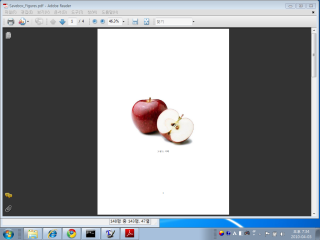
\includegraphics[width=4cm]{fig1}}

\LongText \LongText
\end{boxedverbatim}

\medskip

\ksinsbox[r][2]{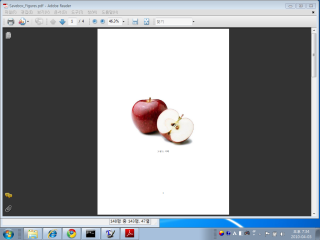
\includegraphics[width=4cm]{fig1}}%

\LongText
\LongText

\paragraph{행 사이에 들어가는 그림}

이를 이용하면 문단의 중간에 그림을 넣을 수 있다. 다만 그림 주위를 텍스트가 흐르지는 않는다. 그 대신 앞 문단을 종료하지 않고도 행 사이에 그림을 넣을 수 있다.
다음 예를 보라.

\bigskip

\begin{boxedverbatim}
\LongText
\ksinsbox[c]{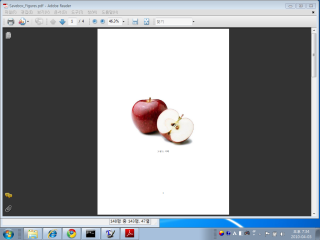
\includegraphics[width=4cm]{fig1}}
\par\LongText
\end{boxedverbatim}

\LongText
\ksinsbox[c]{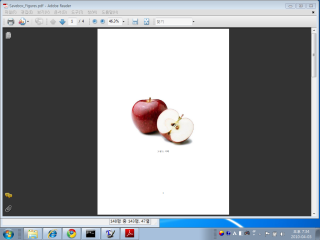
\includegraphics[width=4cm]{fig1}}
\par\LongText


\end{document}
